\documentclass[12pt, fullpage,letterpaper]{article}

\usepackage[margin=1in]{geometry}
\usepackage{url}
\usepackage{amsmath}
\usepackage{amssymb}
\usepackage{xspace}
\usepackage{graphicx}
\usepackage{hyperref}
\usepackage{listings}

\newcommand{\semester}{Fall 2021}
\newcommand{\assignmentId}{2}
\newcommand{\releaseDate}{28 Sep, 2021}
\newcommand{\dueDate}{11:59pm, 19 Oct, 2021}

\newcommand{\bx}{{\bf x}}
\newcommand{\bw}{{\bf w}}

\title{CS 5350/6350: Machine Learining \semester}
\author{Homework \assignmentId}
\date{Handed out: \releaseDate\\
	Due: \dueDate}


\title{CS 5350/6350: Machine Learning \semester}
\author{Homework \assignmentId}
\date{Handed out: \releaseDate\\
  Due date: \dueDate}

\begin{document}
\maketitle

% Math commands by Thomas Minka
\newcommand{\var}{{\rm var}}
\newcommand{\Tr}{^{\rm T}}
\newcommand{\vtrans}[2]{{#1}^{(#2)}}
\newcommand{\kron}{\otimes}
\newcommand{\schur}[2]{({#1} | {#2})}
\newcommand{\schurdet}[2]{\left| ({#1} | {#2}) \right|}
\newcommand{\had}{\circ}
\newcommand{\diag}{{\rm diag}}
\newcommand{\invdiag}{\diag^{-1}}
\newcommand{\rank}{{\rm rank}}
% careful: ``null'' is already a latex command
\newcommand{\nullsp}{{\rm null}}
\newcommand{\tr}{{\rm tr}}
\renewcommand{\vec}{{\rm vec}}
\newcommand{\vech}{{\rm vech}}
\renewcommand{\det}[1]{\left| #1 \right|}
\newcommand{\pdet}[1]{\left| #1 \right|_{+}}
\newcommand{\pinv}[1]{#1^{+}}
\newcommand{\erf}{{\rm erf}}
\newcommand{\hypergeom}[2]{{}_{#1}F_{#2}}

% boldface characters
\renewcommand{\a}{{\bf a}}
\renewcommand{\b}{{\bf b}}
\renewcommand{\c}{{\bf c}}
\renewcommand{\d}{{\rm d}}  % for derivatives
\newcommand{\e}{{\bf e}}
\newcommand{\f}{{\bf f}}
\newcommand{\g}{{\bf g}}
\newcommand{\h}{{\bf h}}
%\newcommand{\k}{{\bf k}}
% in Latex2e this must be renewcommand
\renewcommand{\k}{{\bf k}}
\newcommand{\m}{{\bf m}}
\newcommand{\mb}{{\bf m}}
\newcommand{\n}{{\bf n}}
\renewcommand{\o}{{\bf o}}
\newcommand{\p}{{\bf p}}
\newcommand{\q}{{\bf q}}
\renewcommand{\r}{{\bf r}}
\newcommand{\s}{{\bf s}}
\renewcommand{\t}{{\bf t}}
\renewcommand{\u}{{\bf u}}
\renewcommand{\v}{{\bf v}}
\newcommand{\w}{{\bf w}}
\newcommand{\x}{{\bf x}}
\newcommand{\y}{{\bf y}}
\newcommand{\z}{{\bf z}}
%s\newcommand{\l}{\boldsymbol{l}}
\newcommand{\A}{{\bf A}}
\newcommand{\B}{{\bf B}}
\newcommand{\C}{{\bf C}}
\newcommand{\D}{{\bf D}}
\newcommand{\E}{{\bf E}}
\newcommand{\F}{{\bf F}}
\newcommand{\G}{{\bf G}}
\renewcommand{\H}{{\bf H}}
\newcommand{\I}{{\bf I}}
\newcommand{\J}{{\bf J}}
\newcommand{\K}{{\bf K}}
\renewcommand{\L}{{\bf L}}
\newcommand{\M}{{\bf M}}
\newcommand{\N}{\mathcal{N}}  % for normal density
%\newcommand{\N}{{\bf N}}
\renewcommand{\O}{{\bf O}}
\renewcommand{\P}{{\bf P}}
\newcommand{\Q}{{\bf Q}}
\newcommand{\R}{{\bf R}}
\renewcommand{\S}{{\bf S}}
\newcommand{\T}{{\bf T}}
\newcommand{\U}{{\bf U}}
\newcommand{\V}{{\bf V}}
\newcommand{\W}{{\bf W}}
\newcommand{\X}{{\bf X}}
\newcommand{\Y}{{\bf Y}}
\newcommand{\Z}{{\bf Z}}

% this is for latex 2.09
% unfortunately, the result is slanted - use Latex2e instead
%\newcommand{\bfLambda}{\mbox{\boldmath$\Lambda$}}
% this is for Latex2e
\newcommand{\bfLambda}{\boldsymbol{\Lambda}}

% Yuan Qi's boldsymbol
\newcommand{\bsigma}{\boldsymbol{\sigma}}
\newcommand{\balpha}{\boldsymbol{\alpha}}
\newcommand{\bpsi}{\boldsymbol{\psi}}
\newcommand{\bphi}{\boldsymbol{\phi}}
\newcommand{\boldeta}{\boldsymbol{\eta}}
\newcommand{\Beta}{\boldsymbol{\eta}}
\newcommand{\btau}{\boldsymbol{\tau}}
\newcommand{\bvarphi}{\boldsymbol{\varphi}}
\newcommand{\bzeta}{\boldsymbol{\zeta}}

\newcommand{\blambda}{\boldsymbol{\lambda}}
\newcommand{\bLambda}{\mathbf{\Lambda}}
\newcommand{\bOmega}{\mathbf{\Omega}}
\newcommand{\bomega}{\mathbf{\omega}}
\newcommand{\bPi}{\mathbf{\Pi}}

\newcommand{\btheta}{\boldsymbol{\theta}}
\newcommand{\bpi}{\boldsymbol{\pi}}
\newcommand{\bxi}{\boldsymbol{\xi}}
\newcommand{\bSigma}{\boldsymbol{\Sigma}}

\newcommand{\bgamma}{\boldsymbol{\gamma}}
\newcommand{\bGamma}{\mathbf{\Gamma}}

\newcommand{\bmu}{\boldsymbol{\mu}}
\newcommand{\1}{{\bf 1}}
\newcommand{\0}{{\bf 0}}

% \newcommand{\comment}[1]{}

\newcommand{\bs}{\backslash}
\newcommand{\ben}{\begin{enumerate}}
\newcommand{\een}{\end{enumerate}}

 \newcommand{\notS}{{\backslash S}}
 \newcommand{\nots}{{\backslash s}}
 \newcommand{\noti}{{\backslash i}}
 \newcommand{\notj}{{\backslash j}}
 \newcommand{\nott}{\backslash t}
 \newcommand{\notone}{{\backslash 1}}
 \newcommand{\nottp}{\backslash t+1}
% \newcommand{\notz}{\backslash z}

\newcommand{\notk}{{^{\backslash k}}}
%\newcommand{\noti}{{^{\backslash i}}}
\newcommand{\notij}{{^{\backslash i,j}}}
\newcommand{\notg}{{^{\backslash g}}}
\newcommand{\wnoti}{{_{\w}^{\backslash i}}}
\newcommand{\wnotg}{{_{\w}^{\backslash g}}}
\newcommand{\vnotij}{{_{\v}^{\backslash i,j}}}
\newcommand{\vnotg}{{_{\v}^{\backslash g}}}
\newcommand{\half}{\frac{1}{2}}
\newcommand{\msgb}{m_{t \leftarrow t+1}}
\newcommand{\msgf}{m_{t \rightarrow t+1}}
\newcommand{\msgfp}{m_{t-1 \rightarrow t}}

\newcommand{\proj}[1]{{\rm proj}\negmedspace\left[#1\right]}
\newcommand{\argmin}{\operatornamewithlimits{argmin}}
\newcommand{\argmax}{\operatornamewithlimits{argmax}}

\newcommand{\dif}{\mathrm{d}}
\newcommand{\abs}[1]{\lvert#1\rvert}
\newcommand{\norm}[1]{\lVert#1\rVert}

%miscellaneous symbols
\newcommand{\ie}{{{i.e.,}}\xspace}
\newcommand{\eg}{{{\em e.g.,}}\xspace}
\newcommand{\EE}{\mathbb{E}}
\newcommand{\VV}{\mathbb{V}}
\newcommand{\sbr}[1]{\left[#1\right]}
\newcommand{\rbr}[1]{\left(#1\right)}
\newcommand{\cmt}[1]{}



\section{Paper Problems [40 points + 8 bonus]}
\begin{enumerate}
\item~[5 points] We have derived the PAC guarantee for consistent learners (namely, the learners can produce a hypothesis that can 100\% accurately classify the training data). The PAC guarantee is described as follows. Let $H$ be the hypothesis space used by our algorithm. Let $C$ be the concept class we want to apply our learning algorithm to search for a target function in $C$. We have shown that,  with probability at least $1-\delta$, a hypothesis $h\in H$ that is consistent with a training set of $m$ examples will have the generalization error $\mathrm{err}_D(h) < \epsilon$ if 
\[
m > \frac{1}{\epsilon}\big(\log(|H|) + \log\frac{1}{\delta}\big).
\]

\begin{enumerate}
	\item~[2 points] Suppose we have two learning algorithms $L_1$ and $L_2$, which use hypothesis spaces $H_1$ and $H_2$ respectively. We know that $H_1$ is larger than $H_2$, \ie $|H_1| > |H_2|$.
	For each target function in $C$, we assume both algorithms can find a hypothesis consistent with the training data. 
	\begin{enumerate}
		\item~[1 point] According to Occam's Razor principle, which learning algorithm's  result hypothesis do you prefer? Why?
		
		\emph{Answer}
		
		We desire an answer that requires the least amount of data with some minimum level of confidence.
		
		\item~[1 point]  How is this principle reflected in our PAC guarantee? Please use the above inequality to explain why we will prefer the corresponding result hypothesis. 
		
		\emph{Answer}
		
		This principle is reflected in the $log|H|$ term which is monotonic increasing for $|H|>0$, so smaller $|H|$ implies a smaller number of necessary examples $m$.
		
	\end{enumerate}
	\item~[3 points] Let us investigate algorithm $L_1$. Suppose we have $n$ input features, and the size of the hypothesis space used by $L_1$ is $3^n$. Given $n=10$ features, if we want to guarantee a 95\% chance of learning a hypothesis of at least 90\% generalization accuracy, how many training examples at least do we need for $L_1$?\
	
	\emph{Answer}
	
	\[
        |H| = 3^{n}, n=10 => |H|=3^{10}=59,049
	\]
	\[
	    \epsilon=1-0.9=0.1, 1-\delta=0.95 => \delta=0.05
	\]
	\[
	    m>\frac{1}{0.1}*(log|59,049|+log\frac{1}{0.05})
	\]
	\[
	    m>139.8
	\]
	
	Therefore, we require at least 140 training examples.
	
\end{enumerate}

\item~[5 points] In our lecture about AdaBoost algorithm, we introduced the definition of weighted error in each round $t$, 
\[
\epsilon_t = \frac{1}{2} - \frac{1}{2}\big(\sum_{i=1}^m D_t(i) y_i h_t(x_i)\big)
\]
where $D_t(i)$ is the weight of $i$-th training example, and $h_t(x_i)$ is the prediction of the weak classifier learned round $t$. Note that both $y_i$ and $h_t(x_i)$ belong to $\{1, -1\}$. Prove that equivalently,
\[
\epsilon_t = \sum_{y_i \neq h_t(x_i)} D_t(i).
\]

\emph{Answer}

First, note that when $y_i = h_t(x_i)$ then $y_i * h_t(x_i) = 1$, and conversely when $y_i \neq h_t(x_i)$ then $y_i * h_t(x_i) = -1$.

\[
    => \epsilon_t = \frac{1}{2} - \frac{1}{2}\big(\sum_{y_i = h_t(x_i)} D_t(i) - \sum_{y_i \neq h_t(x_i)} D_t(i)\big)
\]

We then note that $\sum_{i=1}^m D_t(i) = 1$, which can be split into: 

\[\sum_{y_i = h_t(x_i)} D_t(i) + \sum_{y_i \neq h_t(x_i)} D_t(i)\]

\[
    => \epsilon_t = \frac{1}{2}\big(\sum_{y_i = h_t(x_i)} D_t(i) + \sum_{y_i \neq h_t(x_i)} D_t(i)\big) - \frac{1}{2}\big(\sum_{y_i = h_t(x_i)} D_t(i) - \sum_{y_i \neq h_t(x_i)} D_t(i)\big)
\]

\[
    = \frac{1}{2}\sum_{y_i = h_t(x_i)} D_t(i) + \frac{1}{2}\sum_{y_i \neq h_t(x_i)} D_t(i) - \frac{1}{2}\sum_{y_i = h_t(x_i)} D_t(i) + \frac{1}{2}\sum_{y_i \neq h_t(x_i)} D_t(i)
\]

\[
    = \sum_{y_i \neq h_t(x_i)} D_t(i).
\]

\item~[20 points] Can you figure out an equivalent linear classifier for the following Boolean functions? Please point out what the weight vector, the bias parameter and the hyperplane are. Note that the hyperplane is determined by an equation. If you cannot find out a  linear classifier, please explain why, and work out some feature mapping such that, after mapping all the inputs of these functions into a higher dimensional space, there is a hyperplane that well separates the inputs; please write down the separating hyperplane in the new feature space. 
	\begin{enumerate}
		\item~[2 point] $f(x_1, x_2, x_3) = x_1 \land \neg x_2 \land \neg x_3$
		
		\emph{Answer}
		
		Based on that logic function, would expect $y=1$ if $x_1-x_2-x_3>=1$. Table 1 results prove that this function works, so the hyperplane is $y=x_1-x_2-x_3-1$ and $bias=-1$, with a weight vector of $[1, -1, -1]$.
		
		\begin{table}
        	\centering
        	\begin{tabular}{ccccc|c}
        		$x_1 $ & $x_2$ & $x_3$ & $y$ & $x_1-x_2-x_3-1$ & $sign$\\ 
        		\hline\hline
        		0 & 0 & 0 & 0 & -1 & 0 \\ \hline
        		0 & 0 & 1 & 0 & -2 & 0 \\ \hline
        		0 & 1 & 0 & 0 & -2 & 0 \\ \hline
        		0 & 1 & 1 & 0 & -3 & 0 \\ \hline
        		1 & 0 & 0 & 1 &  0 & 1 \\ \hline
        		1 & 0 & 1 & 0 & -1 & 0 \\ \hline
        		1 & 1 & 0 & 0 & -1 & 0 \\ \hline
        		1 & 1 & 1 & 0 & -2 & 0 \\ \hline
        	\end{tabular}
        	\caption{Table of answers for 3a.}\label{tb:1}
        \end{table}
		
		\item~[2 point] $f(x_1, x_2, x_3) = \neg x_1 \lor \neg x_2 \lor \neg x_3$ 
		
		\emph{Answer}
		
		Based on that logic function, would expect $y=1$ if $x_1+x_2+x_3<=-2$. Table 2 results prove that this function works, so the hyperplane is $y=2-x_1-x_2-x_3$ and $bias=2$, with a weight vector of $[1, 1, 1]$.
		
		\begin{table}
        	\centering
        	\begin{tabular}{ccccc|c}
        		$x_1 $ & $x_2$ & $x_3$ & $y$ & $2-x_1-x_2-x_3$ & $sign$\\ 
        		\hline\hline
        		0 & 0 & 0 & 1 &  2 & 1 \\ \hline
        		0 & 0 & 1 & 1 &  1 & 1 \\ \hline
        		0 & 1 & 0 & 1 &  1 & 1 \\ \hline
        		0 & 1 & 1 & 1 &  0 & 1 \\ \hline
        		1 & 0 & 0 & 1 &  1 & 1 \\ \hline
        		1 & 0 & 1 & 1 &  0 & 1 \\ \hline
        		1 & 1 & 0 & 1 &  0 & 1 \\ \hline
        		1 & 1 & 1 & 0 & -1 & 0 \\ \hline
        	\end{tabular}
        	\caption{Table of answers for 3b.}\label{tb:1}
        \end{table}
		
		\item~[8 points] $f(x_1, x_2, x_3, x_4) = (x_1 \lor x_2) \land (x_3 \lor x_4)$
		
		\emph{Answer}
		
		Based on that logic function, would expect $y=1$ if $(x_1+x_2)+(x_3+x_4)>=2$, but this doesn't work because if $x_1=x_2=1$ and $x_3=x_4=0$ then $y=1$ instead of $0$. Instead, let's try a feature mapping that multiplies items in each logic parenthetical together, which yields $(x_1+x_2-x_1x_2)+(x_3+x_4-x_3x_4)>=2$. Table 3 results prove that this function works, so the hyperplane is $y=(x_1+x_2-x_1x_2)+(x_3+x_4-x_3x_4)-2$ and $bias=-2$, with a weight vector of $1's$.
		
		\begin{table}
        	\centering
        	\begin{tabular}{cccccc|c}
        		$x_1 $ & $x_2$ & $x_3$ & $x_4$ & $y$ & $2-x_1-x_2-x_3$ & $sign$\\ 
        		\hline\hline
        		0 & 0 & 0 & 0 & 0 & -2 & 0 \\ \hline
        		0 & 0 & 0 & 1 & 0 & -1 & 0 \\ \hline
        		0 & 0 & 1 & 0 & 0 & -1 & 0 \\ \hline
        		0 & 0 & 1 & 1 & 0 & -1 & 0 \\ \hline
        		0 & 1 & 0 & 0 & 0 & -1 & 0 \\ \hline
        		0 & 1 & 0 & 1 & 1 &  0 & 1 \\ \hline
        		0 & 1 & 1 & 0 & 1 &  0 & 1 \\ \hline
        		0 & 1 & 1 & 1 & 1 &  0 & 1 \\ \hline
        		1 & 0 & 0 & 0 & 0 & -1 & 0 \\ \hline
        		1 & 0 & 0 & 1 & 1 &  0 & 1 \\ \hline
        		1 & 0 & 1 & 0 & 1 &  0 & 1 \\ \hline
        		1 & 0 & 1 & 1 & 1 &  0 & 1 \\ \hline
        		1 & 1 & 0 & 0 & 0 & -1 & 0 \\ \hline
        		1 & 1 & 0 & 1 & 1 &  0 & 1 \\ \hline
        		1 & 1 & 1 & 0 & 1 &  0 & 1 \\ \hline
        		1 & 1 & 1 & 1 & 1 &  0 & 1 \\ \hline
        	\end{tabular}
        	\caption{Table of answers for 3c.}\label{tb:1}
        \end{table}
        
		\item ~[8 points] $f(x_1, x_2) = (x_1 \land x_2) \lor (\neg x_1 \land \neg x_2)$
		
		\emph{Answer}
		
		Based on that logic function, would expect $y=1$ if $(x_1+x_2-2)+(-x_1-x_2)>=1$, but this doesn't work because $x_1$ and $x_2$ cancel out, yielding $-3>=1$, which is false. Instead, let's try a feature mapping that squares each parenthetical, yielding $(x_1+x_2-2)^2+(-x_1-x_2)^2>=1$. But this doesn't work when $x_1=0, x_2=1$ because that yields a true statement when it \emph{should} be false. I note that when $x_1=x_2=1$, then $y=3$, so, what if we just up the third term from $-1$ to $-3$ so when $x_1=x_2=1$ would yield $y=1$. Table 4 results prove that this function works, so the hyperplane is $y=(x_1+x_2-2)^2+(-x_1-x_2)^2-3$, which if we expand it becomes $y=2x_1^2+2x_2^2+4x_1x_2-4x_1-4x_2$ and $bias=0$, with a weight vector of $[2, 2, 4, -4, -4]$.
		
		\begin{table}
        	\centering
        	\begin{tabular}{cccc|c}
        		$x_1 $ & $x_2$ & $y$ & $(x_1+x_2-2)^2+(-x_1-x_2)^2-3$ & $sign$\\ 
        		\hline\hline
        		0 & 0 & 1 &  0 & 1 \\ \hline
        		0 & 1 & 0 & -2 & 0 \\ \hline
        		1 & 0 & 0 & -2 & 0 \\ \hline
        		1 & 1 & 1 &  0 & 1 \\ \hline
        	\end{tabular}
        	\caption{Table of answers for 3d.}\label{tb:1}
        \end{table}
	\end{enumerate}
		
	
	\item~[\textbf{Bonus}]~[8 points]  Given two vectors $\x = [x_1,  x_2]$ and $\y=[y_1,  y_2]$, find a feature mapping $\phi(\cdot)$ for each of the following functions, such that the function is equal to the inner product between the mapped feature vectors, $\phi(\x)$ and $\phi(\y)$. For example, $(\x^\top \y)^0 = \phi(\x)^\top \phi(\y)$ where $\phi(\x) = [1]$ and $\phi(\y) = [1]$; $(\x^\top \y)^1 = \phi(\x)^\top \phi(\y)$ where $\phi(\x) = \x$ and $\phi(\y) = \y$. 
	\begin{enumerate}
		\item~[2 points] $(\x^\top \y)^2$
		
		\emph{Answer}
		
		\[
		    (\x^\top \y)^2 = x_1^2y_1^2 + 2x_1y_1x_2y_2 + x_2^2y_2^2
		\]
		\[
            => \phi(\x) = x_1^2\hat{i} + \sqrt{2}x_1x_2\hat{j} + x_2^2\hat{k}
        \]
		\[
            => \phi(\y) = y_1^2\hat{i} + \sqrt{2}y_1y_2\hat{j} + y_2^2\hat{k}
        \]
        
        
		
		\item~[2 points] $(\x^\top \y)^3$
		
		\emph{Answer}
		
		\[
		    (\x^\top \y)^3 = x_1^3y_1^3 + 3x_1^2y_1^2x_2y_2 + 3x_1y_1x_2^2y_2^2 + x_2^3y_2^3
		\]
		\[
            => \phi(\x) = x_1^3\hat{i} + \sqrt{3}x_1^2x_2\hat{j} + \sqrt{3}x_1x_2^2\hat{k} + x_2^3\hat{l}
        \]
		\[
            => \phi(\y) = y_1^3\hat{i} + \sqrt{3}y_1^2y_2\hat{j} + \sqrt{3}y_1y_2^2\hat{k} + y_2^3\hat{l}
        \]
        
		\item~[4 points] $(\x^\top \y)^k$ where $k$ is  any positive integer.  
		
		\emph{Answer}
		
		Seems to possibly correspond to the Binomial Theorem, $(x+y)^n = \sum_{k=0}^n {n \choose k}x^{n-k}y^k$. However, the difference here would be that for $\phi(\a)$ the $n \choose k$ term becomes $\sqrt{n \choose k}$. Will check a few more to be sure.
		
		\[
		    (\x^\top \y)^4 = x_1^4y_1^4 + 4x_1^3y_1^3x_2y_2 + 6x_1^2y_1^2x_2^2y_2^2 + 4x_1y_1x_2^3y_2^3 + x_2^4y_2^4
		\]
		\[
            => \phi(\x) = x_1^4\hat{i} + \sqrt{4}x_1^3x_2\hat{j} + \sqrt{6}x_1^2x_2^2\hat{k} + \sqrt{4}x_1x_2^3\hat{l} + x_2^4\hat{m}
        \]
		\[
            => \phi(\y) = y_1^4\hat{i} + \sqrt{4}y_1^3y_2\hat{j} + \sqrt{6}y_1^2y_2^2\hat{k} + \sqrt{4}y_1y_2^3\hat{l} + y_2^4\hat{m}
        \]
        
        \[
		    (\x^\top \y)^5 = x_1^5y_1^5 + 5x_1^4y_1^4x_2y_2 + 10x_1^3y_1^3x_2^2y_2^2 + 10x_1^2y_1^2x_2^3y_2^3 + 5x_1y_1x_2^4y_2^4 + x_2^5y_2^5
		\]
		\[
            => \phi(\x) = x_1^5\hat{i} + \sqrt{5}x_1^4x_2\hat{j} + \sqrt{10}x_1^3x_2^2\hat{k} + \sqrt{10}x_1^2x_2^3\hat{l} + \sqrt{5}x_1x_2^4\hat{m} + x_2^5\hat{n}
        \]
		\[
            => \phi(\y) = y_1^5\hat{i} + \sqrt{5}y_1^4y_2\hat{j} + \sqrt{10}y_1^3y_2^2\hat{k} + \sqrt{10}y_1^2y_2^3\hat{l} + \sqrt{5}y_1y_2^4\hat{m} + y_2^5\hat{n}
        \]
        
        By induction, we can apply the Binomial Theorem to $(\x^\top \y)^k$ with the changes described above. This leads to:
        
        \[
            \phi(\x) = \sum_{i=0}^k \sqrt{k \choose i} x_1^{k-i} x_2^{i} \hat{i}
        \]
        \[
            \phi(\y) = \sum_{i=0}^k \sqrt{k \choose i} y_1^{k-i} y_2^{i} \hat{i}
        \]
		
	\end{enumerate}

\item~[10 points] Suppose we have the training data shown in Table \ref{tb:1}, from which we want to learn a linear regression model, parameterized by a weight vector $\w$ and a bias parameter $b$.  
\begin{table}
	\centering
	\begin{tabular}{ccc|c}
		$x_1 $ & $x_2$ & $x_3$ &  $y$\\ 
		\hline\hline
		1 & -1 & 2 & 1 \\ \hline
		1 & 1 & 3 & 4 \\ \hline
		-1 & 1 & 0 & -1 \\ \hline
		1 & 2 & -4 & -2 \\ \hline
		3 & -1 & -1 & 0\\ \hline
	\end{tabular}
	\caption{Linear regression training data.}\label{tb:1}
\end{table}

\begin{enumerate}
	\item~[1 point] Write down the LMS (least mean square) cost function $J(\w, b)$.
	
	\emph{Answer}
	
	The bias is baked into the weights term, so we just need to extract it from regular $J(\w)$.
	
	\[
	    J(\w) = \sum_{i=1}^m (y_i - \w^\top \x_i)^2
	\]
	\[
	    => J(\w, b) = \sum_{i=1}^m (y_i - \w^\top \x_i - b)^2
	\]
	
	\item~[3 points] Calculate the gradient $\frac{\nabla J}{\nabla \w}$ and $\frac{\nabla J}{\nabla b}$ when $\w = [-1,1,-1]^\top$ and $b = -1$.
	
	\emph{Answer}
	
	Code for solution can be found in Listing 1. The function q5b specifically calculates the gradient for the parameters and data (see Table 5) specified. In this case, we find the gradient to be:
	
	\[
	\frac{dJ}{dw_1} = -22
	\]
	\[
    \frac{dJ}{dw_2} = 16
    \]
    \[
    \frac{dJ}{dw_3} = -56
    \]
    \[
    \frac{dJ}{db} = -10
    \]
	
	\begin{lstlisting}[language=Python, caption=QuestionAnswers.part1]

import numpy as np


def q5b():
    x1 = np.array([1, 1, -1, 1, 3])
    x2 = np.array([-1, 1, 1, 2, -1])
    x3 = np.array([2, 3, 0, -4, -1])
    X = np.array([x1, x2, x3]).T
    y = np.array([1, 4, -1, -2, 0]).T
    w = np.array([-1, 1, -1])
    b = -1
    for j in range(len(w)):
        x_j = X[:, j]
        djdw = calc_djdw(X, y, w, b, x_j)
        print(f'dJ_dw_{j + 1}: {djdw}')
    djdb = calc_djdb(X, y, w, b)
    print(f'dJ_db: {djdb}')


def q5c():
    x1 = np.array([1, 1, -1, 1, 3])
    x2 = np.array([-1, 1, 1, 2, -1])
    x3 = np.array([2, 3, 0, -4, -1])
    y = np.array([1, 4, -1, -2, 0]).T
    y_x1 = -np.dot(x1, y)
    print(f'y_x1: {y_x1}')
    y_x2 = -np.dot(x2, y)
    print(f'y_x2: {y_x2}')
    y_x3 = -np.dot(x3, y)
    print(f'y_x3: {y_x3}')
    
    x1_x1 = -np.dot(x1, x1)
    print(f'x1_x1: {x1_x1}')
    x1_x2 = -np.dot(x1, x2)
    print(f'x1_x2: {x1_x2}')
    x1_x3 = -np.dot(x1, x3)
    print(f'x1_x3: {x1_x3}')

    x2_x1 = -np.dot(x2, x1)
    print(f'x2_x1: {x2_x1}')
    x2_x2 = -np.dot(x2, x2)
    print(f'x2_x2: {x2_x2}')
    x2_x3 = -np.dot(x2, x3)
    print(f'x2_x3: {x2_x3}')

    x3_x1 = -np.dot(x3, x1)
    print(f'x3_x1: {x3_x1}')
    x3_x2 = -np.dot(x3, x2)
    print(f'x3_x2: {x3_x2}')
    x3_x3 = -np.dot(x3, x3)
    print(f'x3_x3: {x3_x3}')


def q5d():
    x1 = np.array([1, 1, -1, 1, 3])
    x2 = np.array([-1, 1, 1, 2, -1])
    x3 = np.array([2, 3, 0, -4, -1])
    X = np.array([x1, x2, x3]).T
    y = np.array([1, 4, -1, -2, 0]).T
    w = np.array([0.0, 0.0, 0.0])
    b = 0
    r = 0.1
    for i in range(5):
        for j in range(len(w)):
            djdw = calc_djdw(X[i], y[i], w, b, X[i, j])
            print(f'round {i + 1}, weight updated {j + 1}: {w[j]} + {r * djdw} = {w[j] + r * djdw}')
            w[j] = w[j] + r * djdw
        djdb = calc_djdb(X[i], y[i], w, b)
        print(f'round {i + 1}, bias updated: {b} + {r * djdb} = {b + r * djdb}')
        b = b + r * djdb
    s = 0
    for k in w:
        print(f'w_{s + 1}: {k}')
        s += 1
    print(f'b: {b}')


def calc_djdw(X, y, w, b, x_j):
    return -np.sum(np.dot((y - np.dot(X, w) - b), x_j))


def calc_djdb(X, y, w, b):
    return -np.sum(y - np.dot(X, w) - b)


def calc_cost(X, y, w, b):
    return 0.5 * np.sum(np.square(y - np.dot(X, w) - b))


	\end{lstlisting}
	
	\item~[3 points] What are the optimal $\w$ and $\b$ that minimize the cost function? 
	
	\emph{Answer}
	
	\[
	    J(\w, b) = \frac{1}{2} \sum_{i=1}^m (y_i - \w^\top \x_i - b)^2
	\]
	\[
        => \frac{dJ}{dw_j} = -\sum_{i=1}^m (y_i - \w^\top \x_i - b)x_{ij},  \frac{dJ}{db} = -\sum_{i=1}^m (y_i - \w^\top \x_i - b)
    \]
    Plugging in the data from Table 5, we see that:
    \[
       \frac{dJ}{db} = -2 + 5w_1 +2 w_2 + 0w_3 + 5b
    \]
    Setting this equal to 0 to minimize,
    \[
        => b = \frac{2}{5} - w_1 - \frac{2}{5}w_2
    \]
    \[
        => \frac{dJ}{dw_j} = -\sum_{i=1}^m (y_i x_{ij} - w_1 x_{i1} x_{ij} - w_2 x_{i2} x_{ij} - w_3 x_{i3} x_{ij} - b x_{ij})
    \]
    \[
        = -\sum_{i=1}^m y_i x_{ij} + w_1\sum_{i=1}^m x_{i1} x_{ij} + w_2\sum_{i=1}^m x_{i2} x_{ij} + w_3\sum_{i=1}^m x_{i3} x_{ij} + b\sum_{i=1}^m x_{ij}
    \]
    Function q5c in Listing 1 will calculate the sums above, giving us:
    \[
        \frac{dJ}{dw_1} = 4 - 13w_1 + 2w_2 + 2w_3 - 2 + 5w_1 + 2w_2 = 2 - 8w_1 + 4w_2 + 2w_3 = 0
    \]
    \[
        \frac{dJ}{dw_2} = -2 + 2w_1 - 8w_2 + 6w_3 - \frac{4}{5} + 2w_1 + \frac{4}{5}w_2 = -\frac{14}{5} + 4w_1 - \frac{36}{5}w_2 + 6w_3 = 0
    \]
    \[
        \frac{dJ}{dw_3} = 22 + 2w_1 + 6w_2 - 30w_3 - \frac{4}{5} + 2w_1 + \frac{4}{5}w_2 = -\frac{106}{5} + 4w_1 + \frac{34}{5}w_2 - 30w_3 = 0
    \]
    
    Plugging this system of equations into \href{https://www.wolframalpha.com/input/?i=systems+of+equations+calculator&assumption=%7B%22F%22%2C+%22SolveSystemOf3EquationsCalculator%22%2C+%22equation1%22%7D+-%3E%222-8a%2B4b%2B2c%22&assumption=%22FSelect%22+-%3E+%7B%7B%22SolveSystemOf3EquationsCalculator%22%7D%7D&assumption=%7B%22F%22%2C+%22SolveSystemOf3EquationsCalculator%22%2C+%22equation2%22%7D+-%3E%22-14%2F5%2B4a-36%2F5b%2B6c%22&assumption=%7B%22F%22%2C+%22SolveSystemOf3EquationsCalculator%22%2C+%22equation3%22%7D+-%3E%22106%2F5%2B4a%2B34%2F5b-30c%22}{Wolfram Alpha} (click for link), we get that:
    \[
        w_1 = \frac{247}{223}
    \]
    \[
        w_2 = \frac{258}{223}
    \]
    \[
        w_3 = \frac{249}{223}
    \]
    Which, plugging this back into our equation for $b$, we see that:
    \[
        b = -1.17
    \]
	
	\item~[3 points] Now, we want to use stochastic gradient descent to minimize $J(\w, b)$. We initialize $\w = \0$ and $b = 0$. We set the learning rate $r = 0.1$ and sequentially go through the $5$ training examples. Please list the stochastic gradient in each step and the updated $\w$ and $b$. 
	
	\emph{Answer}
	
	Function q5d in Listing 1 gives these results:
	
	\emph{Round 1}:
	
	weight updated 1: $0.0 + -0.1 = -0.1$
	
	weight updated 2: $0.0 + 0.1100 = 0.1100$
    
    weight updated 3: $0.0 + -0.242 = -0.242$
    
    bias updated: $0 + -0.1694 = -0.1694$
    
    \emph{Round 2}:
    
    weight updated 1: $-0.1 + -0.4885 = -0.5885$
    
    weight updated 2: $0.1100 + -0.5374 = -0.4274$
    
    weight updated 3: $-0.2420 + -1.7734 = -2.0154$
    
    bias updated: $-0.1694 + -1.1232 = -1.2926$
    
    \emph{Round 3}:
    
    weight updated 1: $-0.5885 + 0.0131 = -0.5754$
    
    weight updated 2: $-0.4274 + -0.0145 = -0.4418$
    
    weight updated 3: $-2.0154 + -0.0 = -2.0154$
    
    bias updated: $-1.2926 + -0.0159 = -1.3085$
    
    \emph{Round 4}:
    
    weight updated 1: $-0.5754 + 0.7294 = 0.1540$
    
    weight updated 2: $-0.4418 + 1.6047 = 1.1628$
    
    weight updated 3: $-2.0154 + -4.4931 = -6.5085$
    
    bias updated: $-1.3085 + 2.9205 = 1.6121$
    
    \emph{Round 5}:
    
    weight updated 1: $0.1540 + 2.2259 = 2.3799$
    
    weight updated 2: $1.1628 + -1.4098 = -0.2469$
    
    weight updated 3: $-6.5085 + -1.5507 = -8.0593$
    
    bias updated: $1.6121 + 1.7058 = 3.3179$
    
    \emph{Final Results}
    
    $w_1 = 2.3799$
    
    $w_2 = -0.2469$
    
    $w_3 = -8.0593$
    
    $b = 3.3179$
	
\end{enumerate}
\end{enumerate}

\section{Practice [60 points + 10 bonus]}
\begin{enumerate}
	\item~[2 Points] Update your machine learning library. Please check in your implementation of decision trees in HW1 to your GitHub repository. Remember last time you created a folder ``Decision Tree". You can commit your code into that folder. Please also supplement README.md with concise descriptions about how to use your code to learn decision trees (how to call the command, set the parameters, etc). Please create two folders ``Ensemble Learning" and ``Linear Regression''  in the same level as the folder ``Decision Tree''.  
	
	\emph{Answer}
	
	\href{https://github.com/Paul-Wissler/cs-6350-hw2}{Click here for the repository for HW2}. It is not the same as the repository for HW1.

\item~[36 points] We will implement the boosting and bagging algorithms based on decision trees.  Let us test them on the bank marketing dataset in HW1 (bank.zip in Canvas). We use the same approach to convert the numerical features into binary ones. That is, we choose the media (NOT the average) of the attribute values (in the training set) as the threshold, and examine if the feature is bigger (or less) than the threshold.  For simplicity, we treat ``unknown'' as a particular attribute value, and hence we do not have any missing attributes for both training and test.
\begin{enumerate}
	\item~[8 points] Modify your decision tree learning algorithm to learn decision stumps ---  trees with only two levels. Specifically, compute the information gain to select the best feature to split the data. Then for each subset, create a leaf node. Note that your decision stumps must support weighted training examples. Based on your decision stump learning algorithm, implement AdaBoost algorithm. Vary the number of iterations T from $1$ to $500$, and examine the training and test errors. You should report the results in two figures. The first figure shows how the training and test errors vary along with T. The second figure shows  the training and test errors of all the decision stumps learned in each iteration. What can you observe and conclude? You have had the results for a fully expanded decision tree in HW1. Comparing them with Adaboost, what can you observe and conclude?
	
	\emph{Answer}
	
	Figure 1 shows how Adaboost performs, while Figure 2 shows how individual tree stumps perform. Obviously, this shows that Adaboost performs better, converging to some final error after ~100 rounds, while the individual tree stumps continue to oscillate between 20\% and 80\% error. Comparing Figure 1 to HW1 Table 12 (data used to generate test results for q3b), which shows the accuracy of the data, we can infer that Adaboost performs a bit better on Test data, coming to about 10.7\% error rate, while the best performing tree in Table 12 had an error rate of about 11.4\%. More importantly, though, is that Adaboost seems to be better at reliably generating a well-performing tree with more iterations, making it more stable, while the results in HW1 Table 12 clearly show that the results got \emph{worse} with deeper trees due to over-fitting. I.e., Adaboost's primary advantage over a single tree is that it seems less prone to over-fitting.
	
	\begin{figure}[htp]
        \centering
        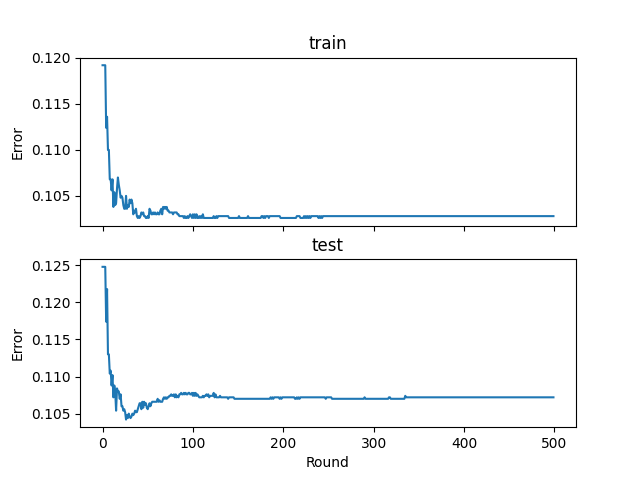
\includegraphics[width=12cm]{q2a_cum_results.png}
        \caption{Training and Test Errors for q2a, Adaboost algorithm after T rounds.}
        \label{fig:q4a}
    \end{figure}
    
    \begin{figure}[htp]
        \centering
        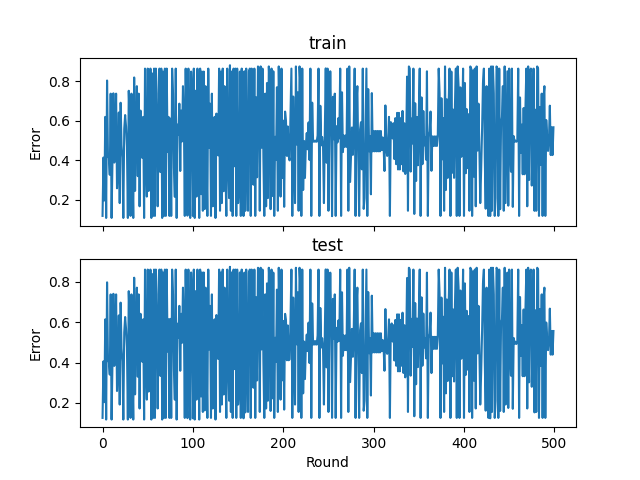
\includegraphics[width=12cm]{q2a_single_results.png}
        \caption{Training and Test Errors for q2a, individual trees over rounds.}
        \label{fig:q4a}
    \end{figure}
	
	\item~[8 points] Based on your code of the decision tree learning algorithm (with information gain), implement a Bagged trees learning algorithm. Note that each tree should be fully expanded --- no early stopping or post pruning. Vary the number of trees from $1$ to $500$, report how the training and test errors vary along with the tree number in a figure. Overall, are bagged trees better than a single tree? Are bagged trees better than Adaboost? 
	
	\emph{Answer}
	
	The results for this question can be found in Figure 3. Based merely on these results, I would say that Adaboost performs better than Bagging, as Adaboost converged to around 10.7\% error on the test data, while bagging converged to around 11.9\%. Interestingly, Adaboost actually had similar performance on both the training and test data, which would indicate that it is less sensitive to over-fitting, while bagging performs better on training data, similar to what we saw with individual trees. The errors still converge, though, making bagging better than single trees. 
	
	However, another interesting note is that the test error was lower on a small number of trees, similar to how a single decision tree with a relatively shallow depth performs better on test data than their full-depth counterparts.
	
	\begin{figure}[htp]
        \centering
        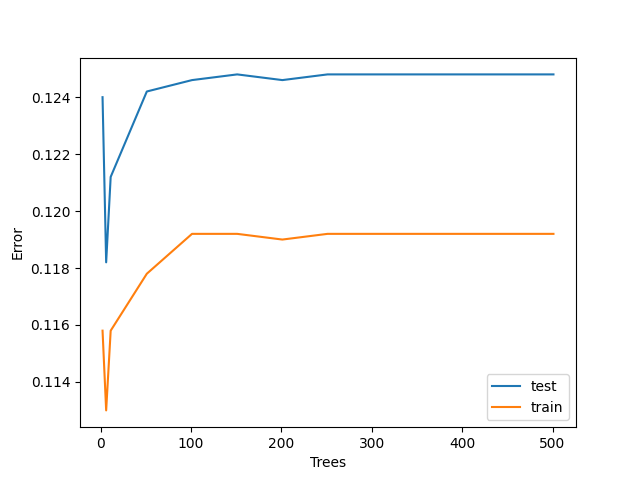
\includegraphics[width=12cm]{q2b_plot.png}
        \caption{Training and Test Errors for q2b.}
        \label{fig:q4a}
    \end{figure}

	\item~[6 points] Through the bias and variance decomposition, we have justified why the bagging approach is more effective than a single classifier/predictor. Let us verify it in real data. Experiment with the following procedure.
	\begin{itemize}
		\item REPEAT for 100 times
		\item ~[STEP 1] Sample $1,000$ examples \textit{uniformly without replacement} from the training datset
		\item ~[STEP 2] Run your bagged trees learning algorithm based on the $1,000$ training examples and learn $500$ trees.
		\item END REPEAT 
		\item Now you have $100$ bagged predictors in hand. For comparison, pick the first tree in each run to get $100$ fully expanded trees (i.e. single trees). 
		\item 	For each of the test example, compute the predictions of the $100$ single trees. Take the average, subtract the ground-truth label, and take square to compute the bias term (see the lecture slides). Use all the predictions to compute the sample variance  as the approximation to the variance term (if you forget what the sample variance is, check it out 
		\href{http://www.randomservices.org/random/sample/Variance.html}{here}). You now obtain the bias and variance terms of a single tree learner for one test example. You will need to compute them for all the test examples and then take average as your final estimate of the bias and variance terms for the single decision tree learner. You can add the two terms to obtain the estimate of the general squared error (that is, expected error w.r.t test examples). Now use your $100$ bagged predictors to do the same thing and estimate the general bias and variance terms, as well as the general squared error.  Comparing the results of the single tree learner and the bagged trees, what can you conclude?  What causes the difference?  
	\end{itemize}
	
	\emph{Answer}
	
	RESULTS:
	
	Single Tree Bias: 0.1060

    Single Tree Sample Variance: 0.0462
    
    Single Tree General Squared Error: 0.1395
    
    Bagged Trees Bias: 0.1246864
    
    Bagged Trees Sample Variance: 0.0001
    
    Bagged Trees General Squared Error: 0.1248
    
    From these results, it seems that the general squared error for Bagged Trees is a bit better than Single Trees. However, Bagged Trees are considerably more biased, but with much smaller variance. From this, I would conclude that Bagged Trees are a more reliable way to make models than single trees. I would be curious to see how limiting tree depth changes Bagged Trees General Squared Error. Based on what I have seen with full-depth trees in HW1, I would expect the General Squared Error to decrease.
	 
	\item~[8 points] Implement the random forest algorithm as we discussed in our lecture. Vary the number of random trees from $1$ to $500$. Note that you need to modify your tree learning algorithm to randomly select a subset of features before each split. Then use the information gain to select the best feature to split.  Vary the size of the feature subset from $\{2, 4, 6\}$.  Report in a figure how the training and test errors vary along with the number of random trees for each feature subset size setting. How does the performance compare with bagged trees? 
	
	\emph{Answer}
	
	Figure 4 shows how well the Random Forest performed. Based merely on these results, I would say that bagging performs better, likely because it has more data to work with when creating its trees, while Random Forests limit themselves to a small number of attributes. To be specific, on test data, bagging error converged to around 12.5\% error, while with 4 and 6 attributes sampled, Random Forests converged to around 13\% error. However, this is not a massive difference, and the error for Random Forests that sample 2 attributes was about 12.5\% as well. There is also the performance to consider, as Random Forests run faster than full bagging based on experience (but with no data to support this claim). 
	
	I take these results with a grain of salt, however, as based on the results seen in q2e, I think that what is happening is that the Random Forest ends up simply taking the mode of the dependent values in training, and assumes all inputs map to that one output. This is most likely a bug with my implementation, but I do not know how to properly fix it.
	
	\begin{figure}[htp]
        \centering
        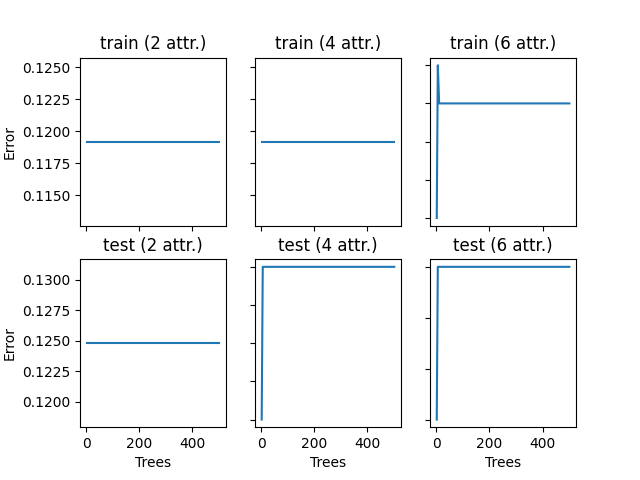
\includegraphics[width=12cm]{q2d_plot.png}
        \caption{Training and Test Errors for q2d, random forest sampling 2, 4, or 6 attributes.}
        \label{fig:q4a}
    \end{figure}
	
	\item~[6 points] Following (c), estimate the bias and variance terms, and the squared error for a single random tree and the whole forest.  Comparing with the bagged trees, what do you observe? What can you conclude? 
	
	\emph{Answer}
	
	Single Tree Bias: 0.11706194
	
    Single Tree Sample Variance: 0.021604101010101014
    
    Single Tree General Squared Error: 0.13106269212272728
    
    Full Forest Bias: 0.1248
    
    Full Forest Sample Variance: 0.0 LIKELY BECAUSE RANDOM FOREST ONLY PREDICTS 0 ON THE DATA
    
    Full Forest General Squared Error: 0.1248
    
    As we saw in q2c, the Full Forest has a smaller error than Single Trees due to a much smaller variance, but with a higher bias. In this case, however, I do not trust these results as indicated in my answer to q2d. The reason why can be seen in the sample variance for the Full Forest, which is exactly 0. On checking the output results from my Random Forest algorithm, I saw that it predicted the same results every single time, and that result was the mode of the training output values. So, it would seem that my Random Forest ends up predicting the mode for any given input. Based on these results, I conclude that there is likely a bug in my implementation. It is possible that tuning my parameters will yield better results.
    
	
\end{enumerate}

\item~[\textbf{Bonus}][10 points] In practice, to confirm the performance of your algorithm, you need to find multiple datasets for test (rather than one). You need to extract and process data by yourself. Now please use the credit default dataset in UCI repository \href{https://archive.ics.uci.edu/ml/datasets/default+of+credit+card+clients}{https://archive.ics.uci.edu/ml/datasets/default+of+credit+card+clients}. Randomly choose $24000$ examples for training and the remaining $6000$ for test. Feel free to deal with continuous features. Run bagged trees, random forest, and Adaboost with decision stumps algorithms for $500$ iterations. Report in a figure how the training and test errors vary along with the number of iterations, as compared with a fully expanded single decision tree. Are the results consistent with the results you obtained from the bank dataset?

\emph{Answer}

\begin{figure}[htp]
    \centering
    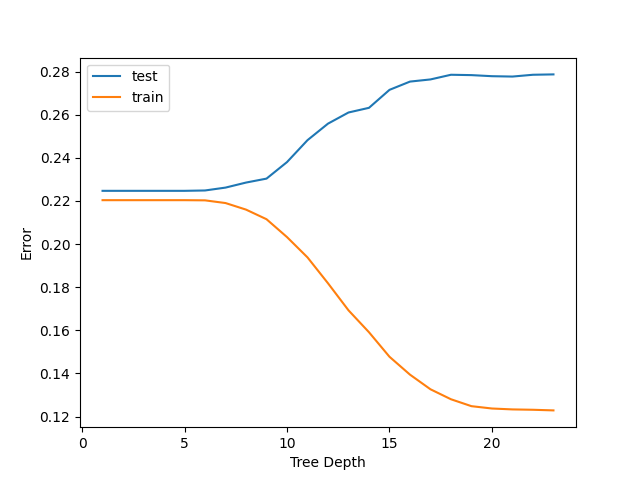
\includegraphics[width=12cm]{q3_decision_tree_plot.png}
    \caption{Decision tree performance on credit default data for q3.}
    \label{fig:q4a}
\end{figure}

\begin{figure}[htp]
    \centering
    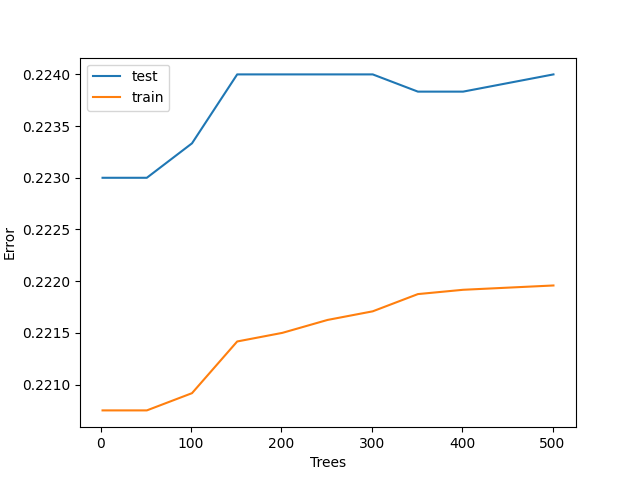
\includegraphics[width=12cm]{q3_adaboost_plot.png}
    \caption{Adaboost performance on credit default data for q3.}
    \label{fig:q4a}
\end{figure}

\begin{figure}[htp]
    \centering
    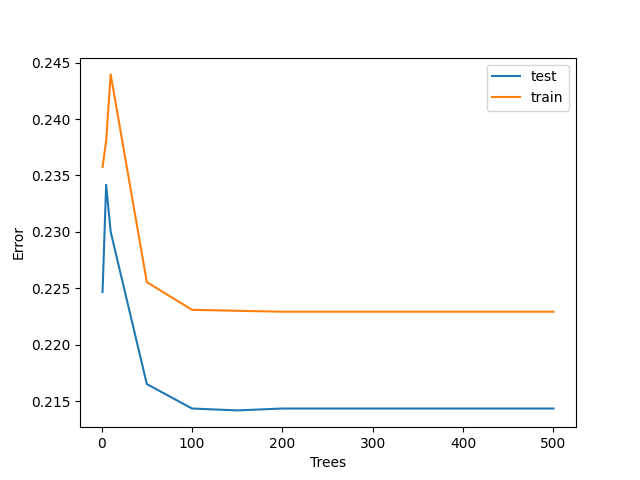
\includegraphics[width=12cm]{q3_bagger_plot.png}
    \caption{Bagger performance on credit default data for q3.}
    \label{fig:q4a}
\end{figure}

\begin{figure}[htp]
    \centering
    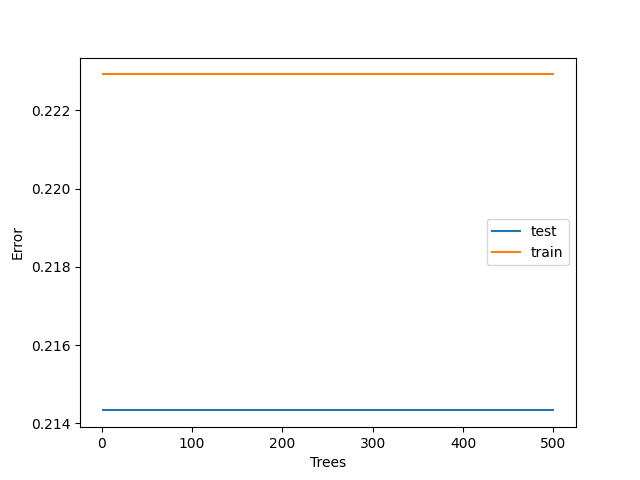
\includegraphics[width=12cm]{q3_random_forest_plot.png}
    \caption{Random forest performance on credit default data for q3.}
    \label{fig:q4a}
\end{figure}

	\item~[22 points] We will implement the LMS method for a linear regression task. The dataset is from UCI repository (\url{https://archive.ics.uci.edu/ml/datasets/Concrete+Slump+Test}). The task is to predict the real-valued SLUMP of the concrete, with $7$ features. The features and output are listed in the file ``concrete/data-desc.txt''. The training data are stored in the file ``concrete/train.csv'', consisting of $53$ examples. The test data are stored in ``concrete/test.csv'', and comprise of $50$ examples. In both the training and testing datasets, feature values and outputs are separated by commas. 
	
	\begin{enumerate}
		\item~[8 points] Implement the batch gradient descent algorithm, and tune the learning rate $r$ to ensure the algorithm converges.  To examine convergence, you can watch the norm of the weight vector difference,  $\|w_{t} - w_{t-1}\|$,  at each step $t$.  if $\|w_{t} - w_{t-1}\|$ is  less than a tolerance level, say, $10^{-6}$, you can conclude that it converges. You can initialize your weight vector to be $\0$.  Please find an appropriate $r$ such that the algorithm converges. To tune $r$, you can start with a relatively big value, say, $r=1$, and then gradually decrease $r$, say $r=0.5, 0.25, 0.125, \ldots$, until you see the convergence. 
		Report the learned weight vector, and the learning rate $r$. Meanwhile, please record the cost function  value of the training data at each step, and then draw a figure shows how the cost function changes along with steps. Use your final weight vector to calculate  the cost function value of the test data. 
		%To do so, you can start $r$ to be relatively big, say, $r=1$, and then gradually decrease $r$. For a specific setting of $r$, you can calculate the cost function after each update and draw a curve showing how the cost function changes along with the number of updates. If you find the cost function on your curve tends to converge, you can conclude your algorithm convergences. 
		
		\emph{Answer}
		
		TEST COST: 41.10059112261912
    
        LEARNING RATE: 0.01
    
        WEIGHT VECTOR
        
        Cement        0.900225
        
        Slag          0.785943
        
        FlyAsh        0.850665
        
        Water         1.298623
        
        SP            0.129834
        
        CoarseAggr    1.571793
        
        FineAggr      0.998347
        
        MODEL\_BIAS   -0.015204
        
        \begin{figure}[htp]
            \centering
            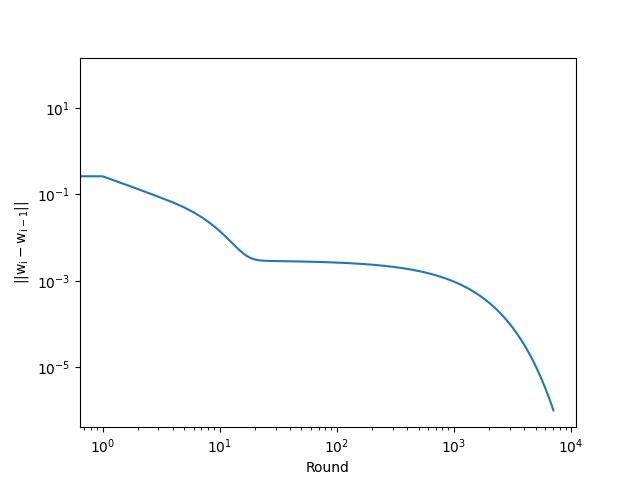
\includegraphics[width=12cm]{part2_q4a.png}
            \caption{Weight convergence with increasing rounds for q4a.}
            \label{fig:q4a}
        \end{figure}
		
		\item~[8 points] Implement the stochastic gradient descent (SGD) algorithm. You can initialize your weight vector to be $\0$. Each step, you randomly sample a training example, and then calculate the stochastic gradient to update the weight vector.  Tune the learning rate $r$ to ensure your SGD converges. To check convergence, you can calculate the cost function of the training data after each stochastic gradient update, and draw a figure showing how the cost function values vary along with the number of updates. At the beginning, your curve will oscillate a lot. However, with an appropriate $r$, as more and more updates are finished, you will see the cost function tends to converge. Please report the learned weight vector, and the learning rate you chose, and the cost function value of the test data with your learned weight vector.
		
		TEST COST: 41.04846572489124
		
		LEARNING RATE: 0.0005
    
        WEIGHT VECTOR
        
        Cement        0.030679
        
        Slag         -0.130154
        
        FlyAsh       -0.127862
        
        Water         0.262171
        
        SP           -0.024053
        
        CoarseAggr    0.058613
        
        FineAggr     -0.018950
        
        MODEL\_BIAS   -0.015117
        
         \begin{figure}[htp]
            \centering
            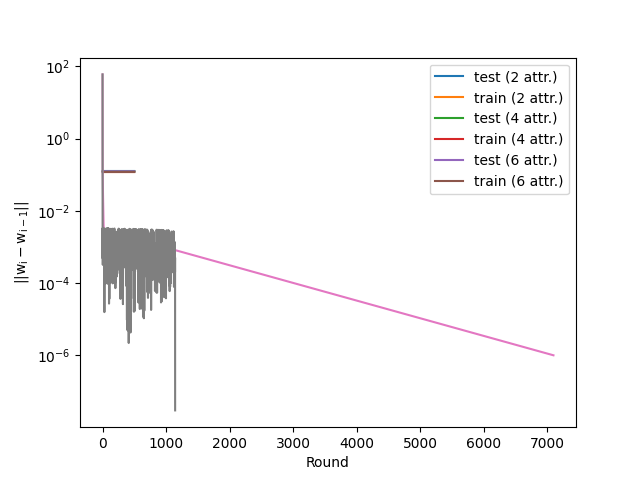
\includegraphics[width=12cm]{part2_q4b.png}
            \caption{Weight convergence with increasing rounds for q4b.}
            \label{fig:q4a}
        \end{figure}
		
		\item~[6 points] We have discussed how to  calculate the optimal weight vector with an analytical form. Please calculate the optimal weight vector in this way. Comparing with the  weight vectors learned by batch gradient descent and stochastic gradient descent, what can you conclude? Why?
		
		\emph{Answer}
		
		Used the code in Listing 2 to calculate the optimal weights from the input X and y.
		
		\begin{lstlisting}[language=Python, caption=Optimal Weights Function]

def calc_optimal_weights(X: pd.DataFrame, y: pd.Series
        ) -> pd.Series:
    X['MODEL_BIAS'] = 1
    nX = X.to_numpy().T # Has to be transposed 
                        # for lin. alg. to work
    ny = y.to_numpy()
    x_xt = np.matmul(nX, np.transpose(nX))
    x_xt_inv = np.linalg.inv(x_xt)
    x_xt_inv_x = np.matmul(x_xt_inv, nX)
    x_xt_inv_x_y = np.dot(x_xt_inv_x, ny)
    return pd.Series(
        x_xt_inv_x_y, index=X.columns
    )

	    \end{lstlisting}
		
		WEIGHT VECTOR
		
	    Cement        0.900565
	    
        Slag          0.786293
        
        FlyAsh        0.851043
        
        Water         1.298894
        
        SP            0.129891
        
        CoarseAggr    1.572249
        
        FineAggr      0.998694
        
        MODEL\_BIAS   -0.015197
    
        This weight vector corresponds almost exactly to what we observe from Batch Gradient Descent, but is almost entirely different from the results for Stochastic Gradient Descent except for the Bias. Although the costs were about the same for Batch Gradient Descent and Stochastic Gradient Descent (both ~41), their weight vectors ended up being very different. I have two guesses as to what may have happened. One, the SGD algorithm hits a local minimum. Based on multiple runs, I think this may be possible as SGD does not always converge for me, indicating there may likely be a bug, as I get bad results no matter what parameters I plug into SGD. The other guess I have is based on the very similar costs for SGD and BGD. It may be possible that the bias is the most important term here, since that term alone is essentially the same for all three sets of results (~-0.015), and perhaps the weights are simply "close enough" in both BGD and SGD. One test I think that may be interesting to check would be to use both of these models as linear classifiers, and see how their error rates compare. If the error rates are significantly different, then I would conclude that, yes, my SGD algorithm is simply broken and needs to be fixed. I tend to think that this is the most likely case, and will proceed from here with the assumption that I failed to properly implement SGD.
    
	\end{enumerate}

\end{enumerate}

\end{document}
%%% Local Variables:
%%% mode: latex
%%% TeX-master: t
%%% End:
